\documentclass[12pt]{article}
\usepackage{url}
\usepackage{tikz}
\usepackage{amsmath}
\usepackage{graphicx}
\usetikzlibrary{positioning}

\title{\vspace{-3em}Evolutionary Algorithms for Mechanical Structures}

\author{Tobias Jacob}
\date{\today}

\begin{document}

\maketitle

\begin{abstract}
\centering
I want to develop a program that improves mechanical structures using an evolutionary algorithm.
\end{abstract}

I have always wondered how to simulate continues mechanics and how to use evolutionary Algorithms to solve engineering problems. The evolutionary algorithm is supposed to generate a 2D mechanical structure and then evaluate if it can withstand a certain force.

\begin{figure}[h]
    \centering
    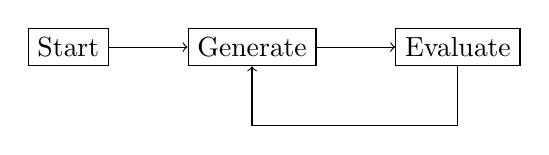
\begin{tikzpicture}
        \node[draw] (start) {Start};
        \node[right=of start, draw] (generate) {Generate};
        \node[right=of generate, draw] (evaluate) {Evaluate};

        \draw[->] (start) -- (generate);
        \draw[->] (generate) -- (evaluate);
        \draw[->] (evaluate) -- +(0, -1cm) -| (generate);
    \end{tikzpicture}
\end{figure}

Each mechanical structure is represented by a 2D boolean array, like the following.

\begin{figure}[h]
    \centering
    \begin{tabular}{cccccc}
        0 & 1 & 1 & 1 & 0 & 0 \\
        0 & 0 & 1 & 0 & 0 & 0 \\
        0 & 0 & 1 & 0 & 0 & 0 \\
        0 & 0 & 1 & 1 & 1 & 0 \\
        0 & 0 & 1 & 1 & 1 & 0 \\
        0 & 0 & 1 & 1 & 1 & 0
    \end{tabular}
\end{figure}

A one is indicating that there is a quadratic element (consisting out of two triangles) present. I may fine tune  The structures get evaluated on withstanding a certain force usinge finite elements. To try out if I am able to implement this, I tried it out in python. With the simplification of using just rectangluar isosceles triangles with side length 1, it is not too complicated. Figure \ref{fig:finiteElements} shows the results of a test python implementation I created. \cite{Nikishkov2004}~has a compact introduction on FEM.

\begin{figure}[h]
    \centering
    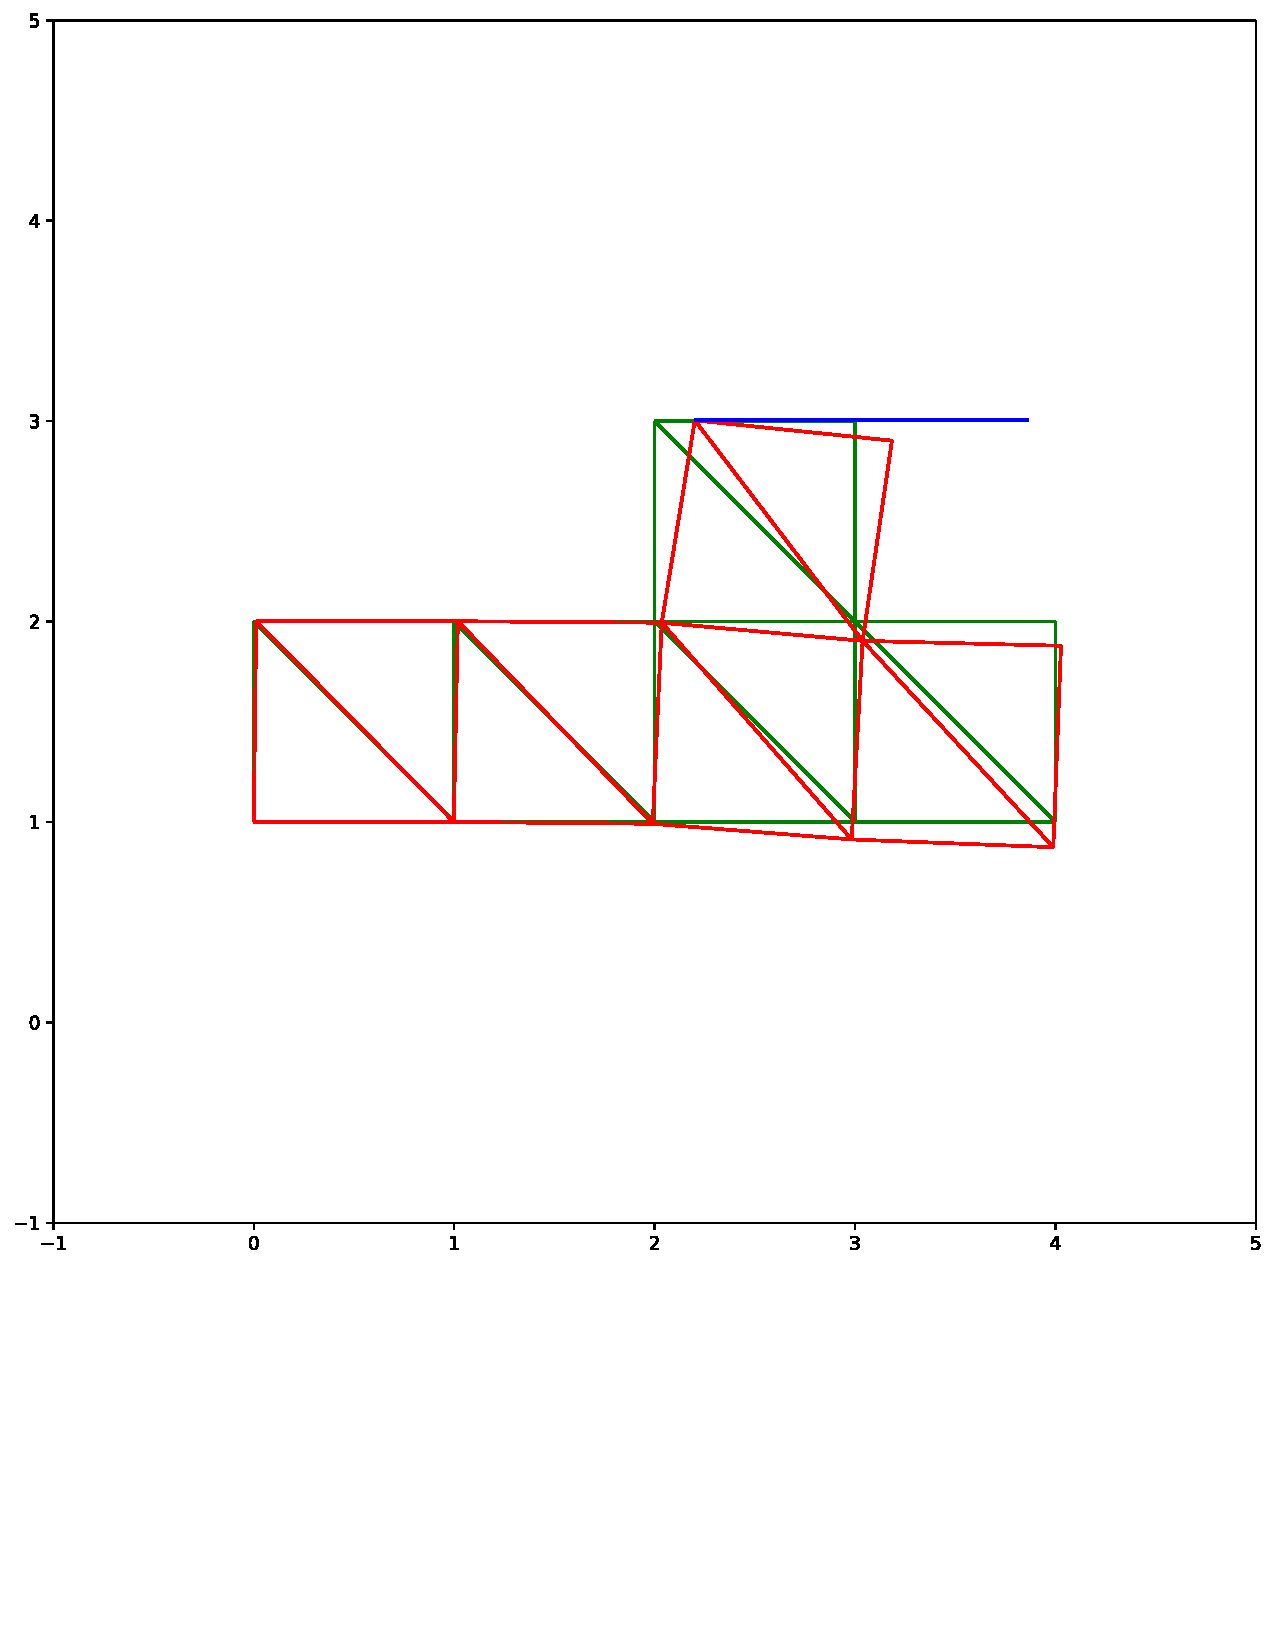
\includegraphics[width=0.5\textwidth]{images/finiteElements.pdf}
    \caption{Example of a finite element simulation}
    \label{fig:finiteElements}
\end{figure}

A bunch of models can be simulated and it can be checked if it can withstand a certain force. Then the best ones get paired and produce children that are similar but have random alterations. After a while, the structures should become more optimized.

Simulating each model can be parallelized. The simulation itself requires solving a linear equation system with a big sparse, symmetric and positive definite matrix. For a 1000x1000 Grid, it would contain $2\cdot 10^6$ elements. After each model has been simulated, all workes must submit their testscores. Then, new models have to be generated and the simulation runs again.


\bibliographystyle{abbrv}
\bibliography{description}

\end{document}
This is never printed